\documentclass[a4paper,11pt]{article}
\usepackage{latexsym}
\usepackage[MeX]{polski}
\usepackage[utf8]{inputenc}
\usepackage[pdftex]{graphicx}

\author{Marcin~Lis}
\title{Projekt {\LaTeX} }
\frenchspacing

\begin{document}
\maketitle
\tableofcontents

\section{Wzory matematyczne}
Przykładowe wzory matematyczne zapisane w {LaTeX} u.

\subsection{Twierdzenie pitagorasa}
\begin{center}
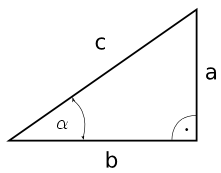
\includegraphics[width=0.3\textwidth]{obrazy/trojkat}
\end{center}
\begin{displaymath}
c^{2}=a^{2}+b^{2}
\end{displaymath}

\subsection{Kombinatoryka}
Kombinatoryka to teoria obliczania liczby elementów zbiorów skończonych. Powstała dzięki grom hazardowym, a swój rozwój zawdzięcza rachunkowi prawdopodobieństwa, teorii grafów, teorii informacji i innym działom matematyki stosowanej. Stanowi jeden z działów matematyki dyskretnej.

Kombinatoryka posługuje się terminologią nie występującą w innych działach matematyki, stąd pozorna jej odrębność. Najważniejszym jej zadaniem jest konstruowanie spełniających pewne określone warunki odwzorowań jednego zbioru skończonego w drugi oraz znajdowanie wzorów na liczbę tych odwzorowań.

\subsubsection{Silnia}
Silnią liczby naturalnej n (w notacji matematycznej: n!, co czytamy „n silnia”) nazywamy iloczyn wszystkich liczb naturalnych nie większych niż n.
\begin{displaymath}
n! =1  \cdot 2 \cdot 3 \cdot \dots \cdot n
\end{displaymath}


\subsubsection{Symbol Newtona}
Symbol Newtona(nazywany też współczynnikiem dwumianowym, czytany n nad k, n po k lub k z n) jest to funkcja dwóch argumentów całkowitych nieujemnych, zdefiniowana jako:
\begin{displaymath}
{n \choose k}=\frac{ n! }{ k!(n-k)! }\quad
\end{displaymath}
gdzie wykrzyknik oznacza silnię.

Wartość symbolu Newtona można wyrazić wzorem rekurencyjnym:
\begin{displaymath}
{n \choose k}= \Bigg\{{1 \atop {n-1 \choose k-1} + {n-1 \choose k} } {dla \  k=0\  lub\  k=1 \atop dla \  0<k<n }
\end{displaymath}

\subsubsection{Wariacje z powtórzeniami}
Wariacją z powtórzeniami k-wyrazową zbioru n-elementowego A nazywa się k-wyrazowy ciąg elementów tego zbioru (dowolny element może wystąpić wielokrotnie w ciągu). Należy zauważyć, iż kolejność elementów ma znaczenie.

Liczba wszystkich k-wyrazowych wariacji z możliwymi powtórzeniami zbioru n-elementowego jest równa:
\begin{displaymath}
\mathrm{V}_n^k=\frac{ n! }{ (n-k)! }\quad
\end{displaymath}
Każda wariacja jest funkcją ze zbioru k-elementowego do zbioru n-elementowego. Funkcje na ogół nie są różnowartościowe. Powtórzenia mogą wystapić, ale nie muszą.

\section{Tabele}
A~tu sie on konczy.

\section{Rysunek}

\end{document}